\documentclass[12pt]{article}

\usepackage{mathtools}
\DeclarePairedDelimiter{\ceil}{\lceil}{\rceil}

\usepackage{amsmath}
\usepackage[margin=1in]{geometry}
\usepackage{enumerate}
\usepackage{amssymb}
\usepackage{amsfonts}
\usepackage{pdfpages}
\usepackage[normalem]{ulem}
\usepackage[pdftitle={ECE 358 Assignment 4},%
pdfsubject={University of Waterloo, ECE 358},%
pdfauthor={Jason Shao, Lihao Luo, Minghao Lu}]{hyperref}

\title{ECE 358 Assignment 4}
\author{Jason Shao, Lihao Luo, Minghao Lu}
\date{June 23, 2016}

\begin{document}
\maketitle
\renewcommand{\thesubsection}{Problem \arabic{subsection}}


\def\question#1{\item[\bf #1.]}
\def\part#1{\item[\bf #1)]}
\newcommand{\pc}[1]{\mbox{\textbf{#1}}} % pseudocode

\begin{enumerate}
	 \item \begin{enumerate}
        \item \begin{enumerate}[(A)]
            \item 1.2.3.0/30
            \item 1.2.3.1
            \item 1.2.3.2
            \item 1.2.3.3
            \item 1.2.3.4/30
            \item 1.2.3.5
            \item 1.2.3.6
            \item 1.2.3.7
            \item 10.1.0.0/16
            \item 10.2.0.0/16
            \item 1.2.3.8/30
            \item 1.2.3.9
            \item 1.2.3.10
            \item 1.2.3.11
            \item 10.3.0.0/16
            \item 10.4.0.0/16
        \end{enumerate}
    \item \begin{enumerate}[(i)]
        \item
            \begin{tabular}{ |c|c|c| } 
             \hline
             Destination & Next Hop & Interface \\ 
             \hline
             1.2.3.4/30 & myself & F \\
             \hline
             1.2.3.0/30 & myself & C \\
             \hline
             0.0.0.0/0 & 1.2.3.1 & C \\
             \hline
            \end{tabular} 
        \item
            \begin{tabular}{ |c|c|c| } 
             \hline
             Destination & Next Hop & Interface \\ 
             \hline
             1.2.3.8/30 & myself & L \\
             \hline
             1.2.3.0/30 & myself & D \\
             \hline
             0.0.0.0/0 & 1.2.3.1 & D \\
             \hline
            \end{tabular} 
        \end{enumerate}
    \end{enumerate}
    
	\item %Q2 Jason
	During the first hop, the MTU is 1000 bytes, but the initial packet is 20 + 1800 = 1820 bytes. Therefor, after fragmentation, $f_1$ will have 20 bytes of header and 976 bytes of payload since the offset has to be a multiple of 8 while maximizing the total packet size to less than 1000 bytes.  Similarly, $f_2$ will have a header of 20 bytes and payload of the remaining 1800 - 976 = 824 bytes (offset of 122). \\ \\ Afterwards, $f_1$ undergoes fragmentation again with MTU of 500 bytes. The first part, $f_1.1$ will have 20 bytes for the header and 480 bytes for payload. The second part, $f_1.2$ will have 20 bytes for the header and 480 bytes for payload (offset of 60). The third part, $f_1.3$ will have 20 bytes for the header and 976 - 480 - 480 = 16 bytes for the payload (offset of 120). \\ \\ In conclusion, the final fragments received at the destination in order of offset is:
	\begin{itemize}
		\item First fragment: ID = abcd, More fragments = 1, Fragment offset = 0, Total length = 500 bytes (480 bytes of payload)
		\item Second fragment: ID = abcd, More fragments = 1, Fragment offset = 60, Total length = 500 bytes (480 bytes of payload)
		\item Third fragment: ID = abcd, More fragments = 1, Fragment offset = 120, Total length = 36 bytes (16 bytes of payload)
		\item Fourth fragment: ID = abcd, More fragments = 0, Fragment offset = 122, Total length = 844 bytes (824 bytes of payload)
	\end{itemize}
	\item %Q3 Jason
	\begin{enumerate}
		\item The header checksum is not necessarily the same, because the TTL field is decremented at each hop, so the header checksum is recomputed at each hop (hence, a different value than the initial checksum).
		\item I do not concur, even if an odd number of bits are flipped, it is not guaranteed to detect an error. A counter-example is 01 FF (checksum FE) because if you flip all nine 1-bits into 0000, the checksum is still FE.
		\item Yes, the UDP checksum at the destination should match that of the source because UDP checksums are end-to-end and is not modified in transit (except when it passes through NAT). 
		\item No, the converse is "if the MTU is supported, you will always get a response" or "if you don't get a response, the MTU is not supported". This is not necessarily true, because there are other reasons for no response other than just a non-supported MTU (such as network congestion or TTL exceeded).
	\end{enumerate}
	\item %Q4 Frank
        Like the assignment suggested, we adopt two premises. 
        (i) at the point in time the slide considers, for every $a \in N'$, $D(a) = d(a)$. 
        (ii) The path $u \rightsquigarrow y$ in the picture, $u \rightsquigarrow x \rightarrow y$,
        is a cheapest path from u to y. Let's call this path $p_1$.\\


        First we prove $D(y) \leq cost(p_1)$. By definition $cost(p_1) = d(x) + c(x,y)$. Since $x \in N'$, 
        by premise (i), $cost(p_1) = D(x) + c(x,y)$. When x was added to $N'$, since y is adjacent to x,
        the algorithm performs $D(y) = min\{D(y), D(x)+c(x,y)\}$, and since the only operations performed on $D(y)$ is to assign
        it a min of its old value and another value, $D(y)$ never increases. Thus $D(y) \leq D(x) + c(x,y)$,
        which combined with $cost(p_1) = D(x) + c(x,y)$, implies $D(y) \leq cost(p_1)$. \\

        Suppose $D(y) \neq d(y)$. Since $d(y)$ is the cheapest cost from u to y, and $D(y)$ is the 
        cost of a path from u to y, $D(y) \geq d(y)$. Since $D(y) \neq d(y)$, $D(y) > d(y)$. 
        Since $d(y) < D(y)$ and $D(y) \leq cost(p_1)$, there must be a path from u to y that is cheaper 
        than $p_1$. But premise (ii) says $p_1$ is a cheapest path from u to y, contradiction. Therefor $D(y) = d(y)$.
        

	\item %Q5 Frank
        
        First we observe $\min_{v \in neigh(x)}\{c(x,v) + d_v(y)\}€6€6€6$
        is at least an upper bound on $d_x(y)$. Let $v_1$ be a neighbour of x that achieves the minimum in
        $\min_{v \in neigh(x)}\{c(x,v) + d_v(y)\}$, i.e $c(x,v_1)+d_{v_1}(y) = \min_{v \in neigh(x)}\{c(x,v) + d_v(y)\}$.  
        Let $v_1 \rightsquigarrow y$ be a minimum path from $v_1$
        to y, i.e. $cost(v_1 \rightsquigarrow y) = d_{v_1}(y)$. Observe $x \rightarrow v_1 \rightsquigarrow y$ is a path from x to y. Moreover
        $cost(x \rightarrow v_1 \rightsquigarrow y) = c(x, v_1) + cost(v_1 \rightsquigarrow y) = c(x, v_1) + d_{v_1}(y) =
        \min_{v \in neigh(x)}\{c(x,v) + d_v(y)\})$.
        Since $d_x(y)$ is the cost of the cheapest path from x to y, 
        $d_x(y) \leq cost(x,v_1 \rightsquigarrow y) = \min_{v \in neigh(x)}\{c(x,v) + d_v(y)\}$. \\

        Suppose $d_x(y) = \min_{v \in neigh(x)}\{c(x,v) + d_v(y)\}$ is not true, since we proved
        $d_x(y) \leq \min_{v \in neigh(x)}\{c(x,v) + d_v(y)\}$, it must be the case 
        $d_x(y) < \min_{v \in neigh(x)}\{c(x,v) + d_v(y)\}$.
        Let $p=x,v_1,v_2,...v_k,y$ be a cheapest path from x to y, then  
        $cost(p) = c(x,v_1) + cost(v_1, v_2,...,v_k,y) < \min_{v \in neigh(x)}\{c(x,v) + d_v(y)\}$. 
        In particular, $c(x, v_1) + cost(v_1,...,v_k,y) < c(x, v_1) + d_{v_1}(y)$,
        which in turn implies $cost(v_1,...,v_k,y) < d_{v_1}(y)$.
        Since $v_1,...,v_k,y$ is a path from $v_1$ to y and $d_{v_1}(y)$ is the cost of the cheapest path from 
        $v_1$ to y, this is a contradiction. Therefor our assumption, $d_x(y) = \min_{v \in neigh(x)}\{c(x,v) + d_v(y)\}$ is not true,
        must be false.

	\item %Q6 Frank

        The number of iterations is the length of a longest of cheapest paths between any two nodes.

        Let $v_1,...,v_k$ be the shortest path between $v_1,...,v_k$ that $v_k$ evetually converges to.  
        First we observe $\forall i \leq k: v_1, v_2, ..., v_i$ is the cheapest path between $v_1$ and $v_i$.
        Suppose its not, then there must be path $v_1,w_1,w_2,...,v_i$ that's shorter , but then \\
        $v_1,w_1,w_2,...,v_i,v_{i+1},v_{i+2},...,v_k$ would be either shorter than $v_1,v_2,...,v_k$.
        Since we defined $v_1,v_2,...,v_k$ as the shortest path between $v_1$ and $v_k$, this is a
        contradiction. Thus $\forall i \leq k: v_1, v_2, ..., v_i$ must be the shortest path between
        $v_1$ and $v_i$. \\

        (For the following section, by "know the cheapest path" I mean know the next hop and total cost) \\

        In an iteration, if $v_i$ doesn't know its cheapest path from $v_1$ yet, since $v_i$ updates its guess of the cheapest
        from $v_1$ path based only on its neighbours guess of cheapest path from $v_1$,
        $v_i$ would and would only learn its true cheapest path from $v_1$ if in the last 
        iteration $v_{i-1}$ knows its true cheapest path from $v_1$. Since by the end of the first iteration, only
        $v_1$ will know its distance for $v_1$, it takes a total of i iterations for $v_i$ to learn
        its true cheapest path from $v_1$. Thus it takes k iterations for $v_k$ to learn its cheapest path
        from $v_1$. \\

        It follows that the number of iterations for everyone to know their cheapest path from everyone else 
        will be the number of nodes in the longest path between any two nodes where that path is also the 
        cheapest path between the two nodes. It's worth noting by the definition of a path, the length is
        bounded by the number of vertices in G, and if G is a linked list, this is simply the number of
        verticies in G.



	\item %Q7 Jason
	\pagebreak
	In figure 1 below, there are 5 nodes in the undirected graph: A, B, C, D, E. The solid lines represent edges and the associated number is the weight of that undirected edge. The dashed line shows that node's minimum weight path to node E. The direction of the dashed line shows the next hop its current min path. 
	\begin{enumerate}[i)]
	\item The first diagram is the initial graph.
	\item The event that causes the Distance Vector protocol to run is the change of weight on edge AE from 1 to 100. Node A is the first to realize this change. It is shown in the second diagram in the figure below.
	\item Diagram 3 - 7 shows one iteration the routing loop, and the chain propagation of shortest path entry updates continues.
	\end{enumerate}
	\pagebreak 
	\begin{figure}[!ht]
    \centering
    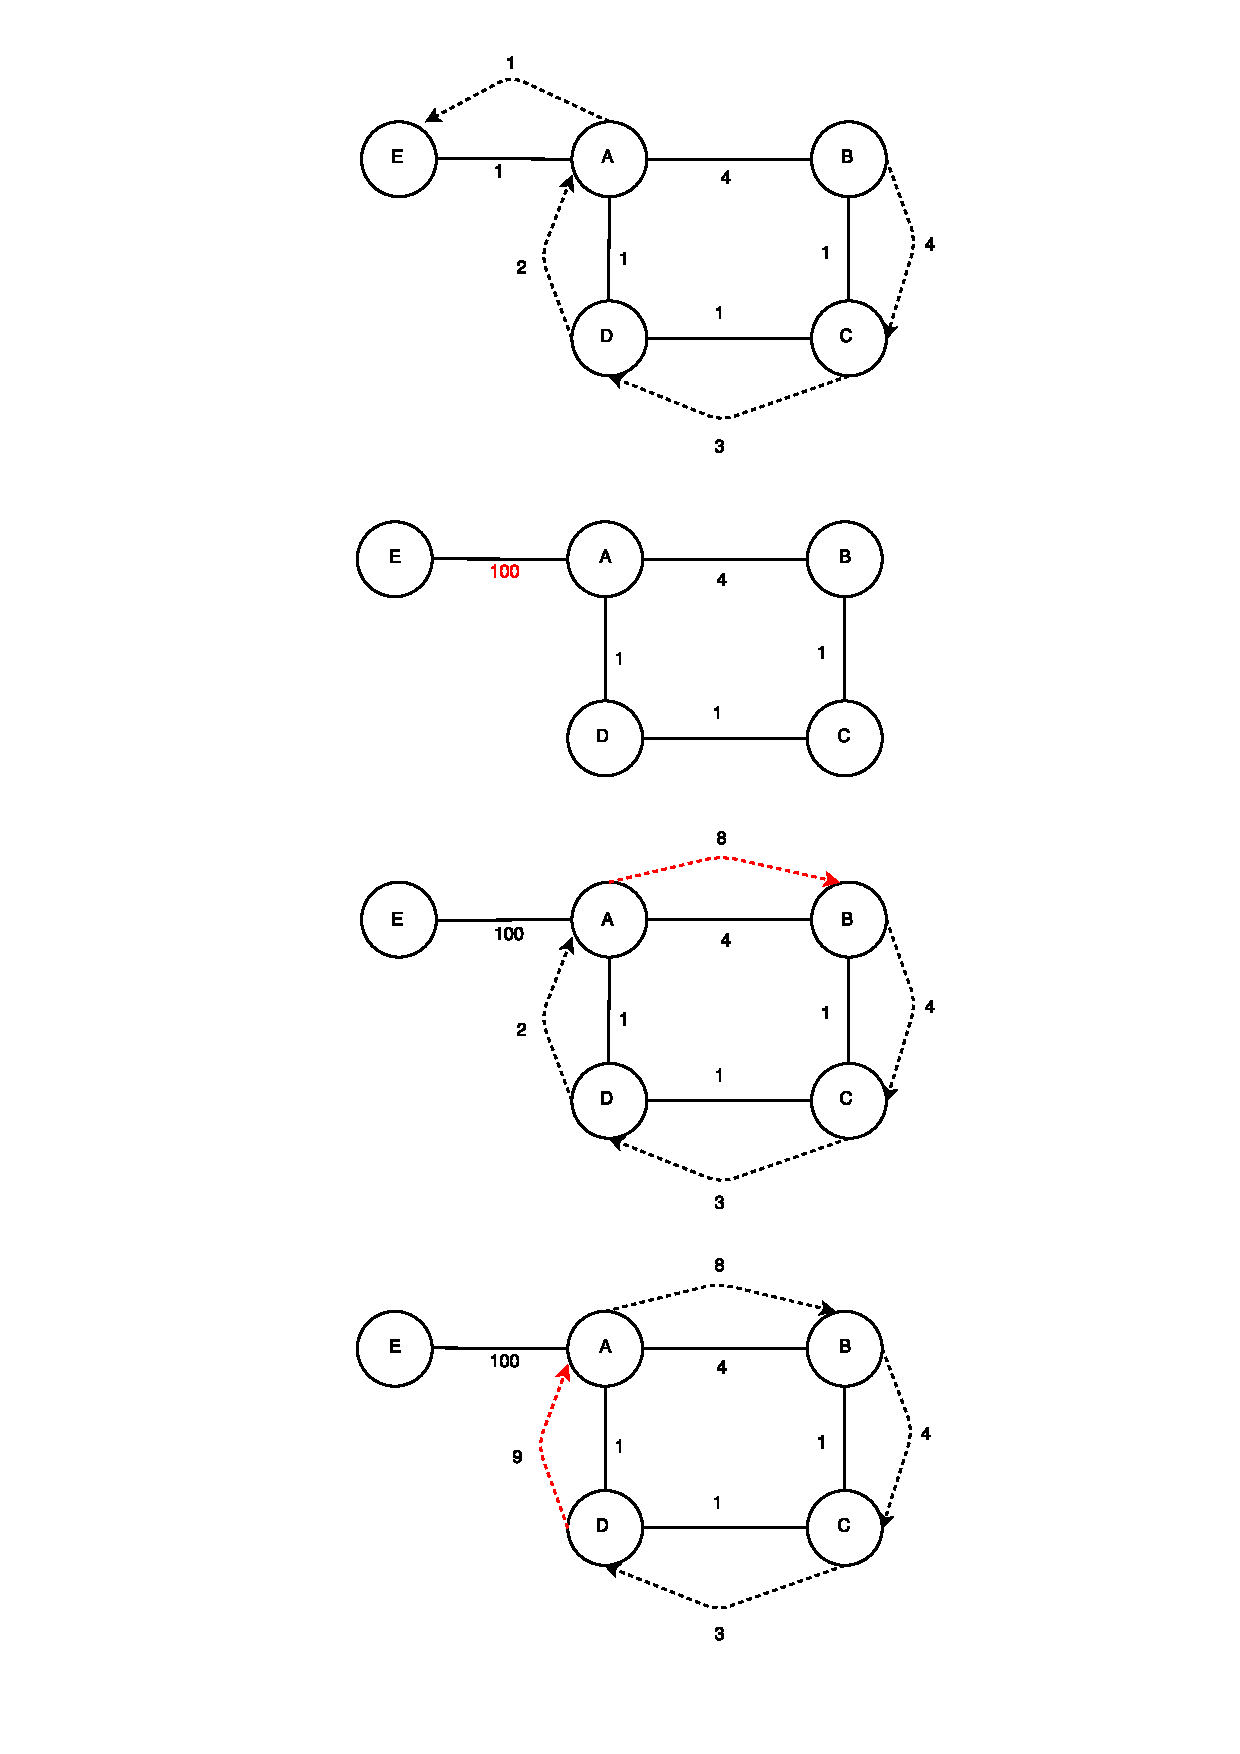
\includepdf[pages={1},scale=0.75]{Poison_Reverse.pdf}
    \caption{Example of routing loop of nodes A, B, C, D}
    \end{figure}
    \pagebreak
	\begin{figure}[!ht]
    \centering
    \includepdf[pages={2},scale=0.75]{Poison_Reverse.pdf}
    %\caption{Example of routing loop of nodes A, B, C, D}
    \end{figure}
\end{enumerate}
\end{document}
